\documentclass[11pt,a4paper]{ctexart}

\usepackage[margin=25mm]{geometry}
\usepackage{amsmath,amssymb}
\usepackage{booktabs}
\usepackage{graphicx}
\usepackage{multirow}
\usepackage{array}
\usepackage{tabularx}
\usepackage{float}
\usepackage{caption}
\usepackage{subcaption}
\usepackage{siunitx}
\usepackage{hyperref}
\usepackage{enumitem}
\usepackage{bm}
\usepackage{xcolor}
\usepackage{colortbl}
\makeatletter
\let\insert@pcolumn\insert@column
\makeatother
\usepackage{tikz}
\usetikzlibrary{arrows.meta,positioning,shapes.geometric,calc}

\definecolor{passgreen}{RGB}{34,139,34}
\definecolor{failred}{RGB}{220,20,60}
\definecolor{warnblue}{RGB}{30,80,180}
\definecolor{lightgray}{RGB}{240,240,240}

\newcommand{\dd}{\mathrm{d}}
\newcommand{\pp}{\partial}
\newcommand{\bsig}{\bm{\sigma}}
\newcommand{\beps}{\bm{\varepsilon}}
\newcommand{\bD}{\bm{D}}
\newcommand{\bB}{\bm{B}}
\newcommand{\bE}{\bm{E}}
\newcommand{\bH}{\bm{H}}

\title{\textbf{含孔隙功能梯度磁--电--弹性板在热--磁--电--弹性全耦合下的\\参数化仿真：孔隙率、梯度分布与体积分数的影响}}
\author{作者}
\date{\today}

\begin{document}
\maketitle

\begin{abstract}
本文针对含孔隙功能梯度磁--电--弹性（FG-MEE）板在热--磁--电--弹性全耦合载荷下的静力与动力响应开展了系统的参数化研究。模型采用基于一阶剪切变形理论（FSDT）的八节点 Serendipity 单元有限元格式，将三种孔隙分布模型（均匀 Even、非均匀 Uneven 和对数非均匀 LogUneven）嵌入厚度方向的材料梯度之中。设计空间组合了两种 FG 分布（均匀 U 型与表面富集 X 型）、五个孔隙率水平（$e_0 = 0$--$0.4$）、三种孔隙模式与五个体积分数；在剔除 $e_0 = 0$ 时三模式等价的重复项后，共得到 130 个材料配置、390 行三载荷（力、电、磁）静力结果。对无孔隙代表工况的 COMSOL Multiphysics 独立校核显示其偏差在 5\% 以内（中心点偏差 3.77\%，15 点最大偏差 4.93\%）；非均匀 V/X 与 CFCF 代表工况也满足该准则，而含孔隙代表工况暴露出 5\% 量级的三维实体等效模型偏差，需要进一步做模型构型复核。主要发现包括：（1）$e_0 = 0.4$ 的均匀孔隙使机械挠度放大约 74\%，同时使压电致动响应降低约 46\%；（2）非均匀（中心富集）孔隙即使在 $e_0 = 0.4$ 时也将挠度增幅限制在约 13\%，保留了大部分弯曲刚度；（3）X 型 FG 分布产生的变形诱导厚度方向温差跨度最小；（4）磁电转化效率随孔隙率单调退化，其中 X-对数非均匀组合退化最强（$e_0 = 0.4$ 时损失 30.4\%）。代表性瞬态 Newmark 分析给出的超调比，无孔隙工况（2.11）与含孔隙工况（2.13）均接近 2.1，表明孔隙不改变阶跃响应的定性特征。上述结果为传感器与致动器应用中的含孔隙 FG-MEE 结构提供了定量设计指导。

\medskip
\noindent\textbf{关键词：} 功能梯度材料；磁电弹耦合；孔隙率；一阶剪切变形；有限元；COMSOL 验证
\end{abstract}

\tableofcontents
\newpage

% ============================================================
\section{研究模型与目标}
% ============================================================

\subsection{研究背景}

磁--电--弹性（Magneto-Electro-Elastic, MEE）复合材料通常由压电相 BaTiO$_3$ 与压磁相 CoFe$_2$O$_4$ 构成，能够同时呈现压电、压磁与磁电耦合效应，在传感器、能量俘获器与微波器件中具有重要应用价值。当两相沿板厚方向以功能梯度（Functionally Graded, FG）方式排布时，所得 FG-MEE 结构可获得均质复合材料无法实现的可调多物理场响应。

近年来，针对 MEE 板的全耦合热--磁--电--弹性有限元模型已经建立，并证实结构变形会通过热弹耦合机制诱导出可观测的温度场变化。然而，已有参数化研究多局限于理想致密材料，忽略了烧结过程中因温度不均、颗粒尺寸失配与界面反应而不可避免产生的微观孔隙。孔隙会显著降低有效弹性模量与耦合系数，从而同时改变机械响应与多物理场耦合行为。本文将孔隙效应引入热--磁--电--弹性全耦合框架，系统考察孔隙率、梯度分布与体积分数对全耦合响应（尤其是变形诱导温度场）的影响。

\subsection{模型概述}

研究对象为含孔隙功能梯度磁--电--弹性方板，在热--磁--电--弹性全耦合条件下的静力与动力响应。板的几何与基本设置见表~\ref{tab:model-params}。

\begin{table}[H]
\centering
\caption{FG-MEE 板模型基本参数}
\label{tab:model-params}
\begin{tabular}{lll}
\toprule
\textbf{参数} & \textbf{取值} & \textbf{说明} \\
\midrule
几何尺寸 & $300\times300\times6$\,mm & 方板 \\
边界条件 & CFFF / CFCF & 单边固支 / 两对边固支 \\
材料组分 & BaTiO$_3$ / CoFe$_2$O$_4$ & 压电相 / 压磁相 \\
FG 分布 & U, V, X, O, P & 5 种梯度模式 \\
体积分数 $V_{f0}$ & 0.1--0.9 & 最多 9 个水平 \\
孔隙率 $e_0$ & 0--0.4 & 5 个水平 \\
孔隙模式 & Even / Uneven / LogUneven & 3 种分布 \\
厚度分层 & 10 层 & 逐层混合律赋值 \\
网格 & $30\times30$ 八节点 Serendipity & 961 节点 / 900 单元 \\
\bottomrule
\end{tabular}
\end{table}

\subsection{研究目标}

本研究拟完成的核心目标如下：
\begin{enumerate}[leftmargin=2em]
\item \textbf{无孔隙静力参数扫描：} 完成 $5\times9\times3=135$ 组静力算例（5 种 FG 分布 $\times$ 9 个体积分数 $\times$ 3 种载荷类型），输出中心挠度、层温差跨度与磁电效率；
\item \textbf{磁电耦合转化验证：} 以 2\,mm 统一参考挠度建立正向驱动（电/磁$\to$位移）与反向传感（位移$\to$电/磁）的双向转化验证体系；
\item \textbf{独立数值验证：} 用 COMSOL Multiphysics 对代表工况独立建模，无孔隙 CFFF、非均匀 V/X 与 CFCF 代表行均满足 5\% 准则，含孔隙代表行作为模型构型复核项记录；
\item \textbf{动力响应分析：} 通过 Newmark-$\beta$ 直接积分与模态降阶，获取瞬态阶跃响应的峰值、超调比与固有频率特征；
\item \textbf{含孔隙扩展：} 将三种孔隙模型嵌入材料梯度，构建 130 配置 / 390 行的含孔隙设计空间，量化孔隙率对刚度、致动能力、温度场与磁电效率的影响规律。
\end{enumerate}

% ============================================================
\section{计算与仿真方法}
% ============================================================

\subsection{MEE 本构方程}

对于横观各向同性 MEE 材料，在线性耦合假设下，采用 Voigt 记法的本构关系为：
\begin{align}
\bsig &= \bm{C}\,\beps - \bm{e}^T\bE - \bm{q}^T\bH - \bm{\lambda}\,\Delta T \label{eq:stress}\\
\bD &= \bm{e}\,\beps + \bm{\chi}\,\bE + \bm{\kappa}\,\bH + \bm{p}_E\,\Delta T \label{eq:D}\\
\bB &= \bm{q}\,\beps + \bm{\kappa}^T\bE + \bm{\gamma}\,\bH + \bm{p}_M\,\Delta T \label{eq:B}\\
\rho c_v \dot{T} &= T_0\left(\bm{\lambda}^T\dot{\beps} + \bm{p}_E^T\dot{\bE} + \bm{p}_M^T\dot{\bH}\right) \label{eq:thermal}
\end{align}
其中 $\bm{C}$ 为弹性刚度矩阵，$\bm{e}$ 与 $\bm{q}$ 分别为压电、压磁系数矩阵，$\bm{\chi}$ 与 $\bm{\gamma}$ 分别为介电常数与磁导率矩阵，$\bm{\kappa}$ 为磁电耦合矩阵，$\bm{\lambda}$ 为热应力模量向量，$\bm{p}_E$ 与 $\bm{p}_M$ 为热释电与热释磁系数，$\rho$ 为质量密度，$c_v$ 为比热容。式~\eqref{eq:thermal} 描述了变形诱导温度场：机械应变率、电场率与磁场率均通过全耦合热弹机制贡献局部温度变化。

\subsection{功能梯度材料分布}

BaTiO$_3$ 的体积分数 $V_f(z)$ 沿板厚按所选 FG 分布变化。对厚度为 $h$、$z \in [-h/2, h/2]$ 的板，定义归一化坐标 $\zeta = z/h + 1/2$（底面 0、顶面 1）与 $\bar{z} = |z|/(h/2)$（中面 0、表面 1）。共考虑五种分布模式：
\begin{equation}
V_f(z) = \begin{cases}
V_{f0} & \text{U 型（均匀）} \\
V_{f0}\,\zeta & \text{V 型（线性）} \\
V_{f0}\,\bar{z} & \text{X 型（表面富集）} \\
V_{f0}\,(2 - \bar{z}) & \text{O 型（中心富集）} \\
V_{f0}\,\zeta^n & \text{P 型（幂律）}
\end{cases}
\label{eq:fg-modes}
\end{equation}
其中 $V_{f0}$ 为名义体积分数参数，$n$ 为幂律指数（本文取 2）。任意高度 $z$ 处的有效材料属性由 Voigt 型线性混合律给出：
\begin{equation}
P_{\text{dense}}(z) = V_f(z)\,P_{\text{BTO}} + [1 - V_f(z)]\,P_{\text{CFO}}
\label{eq:mixture}
\end{equation}
式中 $P$ 表示任一材料常数（$C_{ij}$、$e_{ij}$、$q_{ij}$、$\chi_{ij}$、$\gamma_{ij}$、$\kappa_{ij}$、$\lambda_i$、$\rho$、$c_v$ 等）。

为直观说明上述材料分布，图~\ref{fig:fg-gradient-shell-schematic} 给出了功能梯度板壳的逐层赋值示意。板厚方向被离散为 10 个材料层，每层在层中面取 $V_f(z)$ 并通过混合律换算为一组等效材料常数；梯度本身不作为连续颜色场直接求解，而是通过 10 个层域的材料常数差异体现。右侧曲线显示 U/V/X/O/P 五种 $V_f(z)$ 分布及三种孔隙模式的有效属性保留系数，其中 X 型体现表面富集，O 型体现中心富集，Uneven 孔隙则在中面附近退化最强、表层退化最弱。

\begin{figure}[H]
\centering
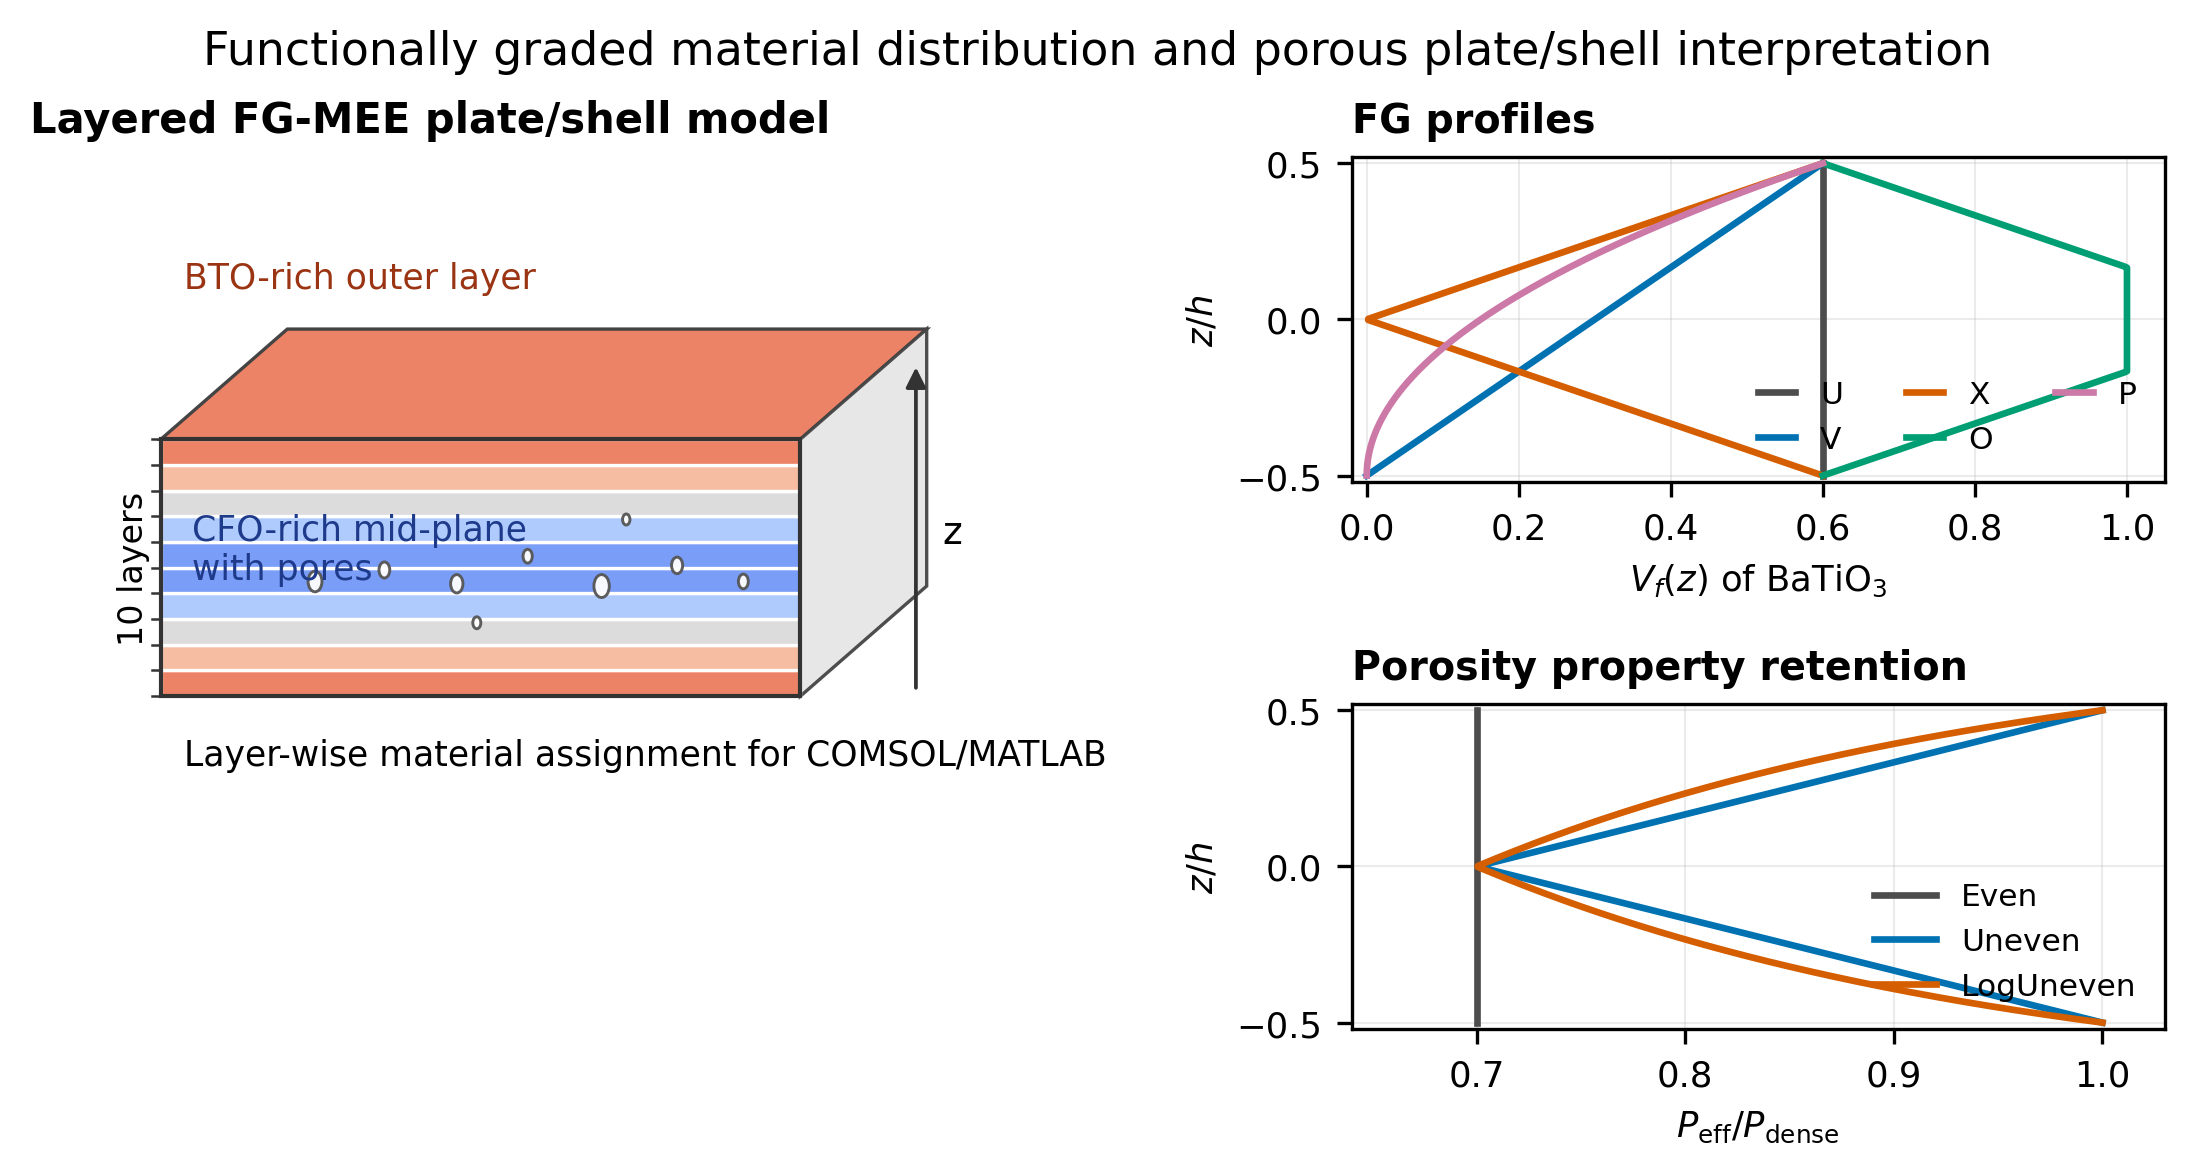
\includegraphics[width=0.95\textwidth]{figures/fg_gradient_shell_schematic.png}
\caption{功能梯度材料分布与含孔隙板壳分层模型示意图}
\label{fig:fg-gradient-shell-schematic}
\end{figure}

\subsection{孔隙修正模型}

实际 FG-MEE 材料因烧结过程含有微观孔隙。本文采用三种孔隙分布模型：

\noindent\textbf{模式 I —— 均匀（Even）孔隙：}
\begin{equation}
P_{\text{eff}}(z) = P_{\text{dense}}(z)\,(1 - e_0)
\label{eq:poro-even}
\end{equation}

\noindent\textbf{模式 II —— 非均匀（Uneven，中心富集）孔隙：}
\begin{equation}
P_{\text{eff}}(z) = P_{\text{dense}}(z)\left[1 - e_0\left(1 - \frac{2|z|}{h}\right)\right]
\label{eq:poro-uneven}
\end{equation}

\noindent\textbf{模式 III —— 对数非均匀（LogUneven）孔隙：}
\begin{equation}
P_{\text{eff}}(z) = P_{\text{dense}}(z) - \frac{e_0}{2}\ln\!\left(\frac{1}{1 - 2|z|/h}\right)\left[V_f(z)\,P_{\text{BTO}} + (1-V_f(z))\,P_{\text{CFO}}\right]
\label{eq:poro-log}
\end{equation}
式中 $e_0 \in (0, 1)$ 为孔隙率参数。模式 I 对所有层施加均匀退化；模式 II 将孔隙集中于板中面而保持表面致密；模式 III 提供介于两者之间的对数过渡。当 $e_0 = 0$ 时三种模式完全等价，因此在设计空间中只保留一份基线。

\subsection{一阶剪切变形板理论与有限元离散}

位移场采用 Mindlin--Reissner 一阶剪切变形理论（FSDT）：
\begin{equation}
\begin{aligned}
u(x,y,z,t) &= u_0(x,y,t) + z\,\psi_x(x,y,t) \\
v(x,y,z,t) &= v_0(x,y,t) + z\,\psi_y(x,y,t) \\
w(x,y,z,t) &= w_0(x,y,t)
\end{aligned}
\label{eq:fsdt}
\end{equation}
其中 $(u_0, v_0, w_0)$ 为中面位移，$(\psi_x, \psi_y)$ 为法线绕 $y$、$x$ 轴的转角。板在 $xy$ 平面内采用八节点 Serendipity 单元离散，每个节点含 5 个机械自由度。电势与磁势在每个材料层内沿厚度线性变化，给出每节点 $(N_L+1)$ 个电自由度与 $(N_L+1)$ 个磁自由度，其中 $N_L$ 为厚度方向层数（本文取 10）。温度场作为由式~\eqref{eq:thermal} 导出的次级（感生）变量。应变--位移关系为 $\beps = \bm{B}_u\,\bm{d}_e$，$\bm{B}_u$ 由形函数 $N_i(\xi,\eta)$ 的导数组装。

\subsection{逐层材料积分与单元矩阵}

板厚被均分为 $N_L = 10$ 个子层。在厚度方向每个 Gauss 点处，由式~\eqref{eq:fg-modes} 计算局部体积分数 $V_f(z_k)$，由式~\eqref{eq:mixture} 计算致密混合属性，再依所选模式由式~\eqref{eq:poro-even}--\eqref{eq:poro-log} 施加孔隙修正。单元刚度矩阵通过沿厚度数值积分组装：
\begin{equation}
\bm{K}_{uu}^e = \int_{\Omega_e}\sum_{k=1}^{N_L}\int_{z_k^-}^{z_k^+} \bm{B}_u^T\,\bm{C}_{\text{eff}}(z)\,\bm{B}_u\;\dd z\;\dd\Omega
\end{equation}
其中 $\bm{C}_{\text{eff}}(z)$ 含孔隙修正后的弹性常数。同理，压电耦合矩阵 $\bm{K}_{u\phi}^e$、压磁耦合矩阵 $\bm{K}_{u\psi}^e$、磁电耦合矩阵 $\bm{K}_{\phi\psi}^e$、热耦合矩阵以及质量矩阵 $\bm{M}_{uu}^e$ 均以各层中面修正后的材料属性计算。

\subsection{耦合系统方程}

\subsubsection{静力分析}

静力全耦合系统为：
\begin{equation}
\begin{bmatrix}
\bm{K}_{uu} & \bm{K}_{u\theta} \\
\bm{K}_{\theta u} & \bm{K}_{\theta\theta}
\end{bmatrix}
\begin{Bmatrix}
\bm{Q}_d \\ \bm{\Theta}_s
\end{Bmatrix}
=
\begin{Bmatrix}
\bm{F}_{\text{ext}} \\ \bm{0}
\end{Bmatrix}
\label{eq:static-system}
\end{equation}
其中 $\bm{Q}_d$ 为机械位移，$\bm{\Theta}_s$ 为感生（变形诱导）温度向量，外载 $\bm{F}_{\text{ext}} = \bm{F}_{\text{mech}} - \bm{K}_{u\phi}\,\bm{\Phi}_a - \bm{K}_{u\psi}\,\bm{\Psi}_a$ 包含机械、电势 $\bm{\Phi}_a$ 与磁势 $\bm{\Psi}_a$ 三类载荷贡献。磁电转化效率定义为 $\alpha_{\text{ME}} = \phi_{\text{out}}/\psi_{\text{in}}$，即施加磁势 $\psi_{\text{in}}$ 经回代得到的感生电势 $\phi_{\text{out}}$ 之比。

\subsubsection{动力分析}

瞬态分析采用 Newmark-$\beta$ 直接积分（$\beta = 1/4$，$\gamma = 1/2$），运动方程为：
\begin{equation}
\bm{M}_{uu}\,\ddot{\bm{Q}}_d + \bm{C}\,\dot{\bm{Q}}_d + \bm{K}_{uu}\,\bm{Q}_d = \bm{F}_{\text{ext}}(t)
\label{eq:newmark}
\end{equation}
其中 $\bm{C} = 2\xi\omega_1\bm{M}_{uu}$ 为 Rayleigh 阻尼矩阵，阶跃载荷 $\bm{F}_{\text{ext}}(t) = \bm{F}_0\,H(t)$，$H(t)$ 为 Heaviside 函数。对 $30\times30$ 网格（约 13800 自由度），采用模态叠加将系统投影至前 $N_m$ 阶特征向量 $\bm{\Phi}_m$（由广义特征值问题 $\bm{K}_{uu}\bm{\Phi}_m = \omega^2\bm{M}_{uu}\bm{\Phi}_m$ 得到），把有效规模从约 13800 降至 $N_m$（通常 8--16 阶即可收敛）。

\subsection{总体技术路线}

整体计算流程如图~\ref{fig:workflow} 所示：从材料混合律与 FG 分布生成出发，经 MATLAB 板壳全耦合 FEM 完成静力扫描与 2\,mm 耦合验证，一路分支至 COMSOL 独立验证，另一路推进至 Newmark 与模态降阶动力分析，最终汇总为无孔隙/非均匀/CFCF 误差 $<5\%$ 与含孔隙模型复核结论。

\begin{figure}[H]
\centering
\begin{tikzpicture}[
  node distance=1.0cm and 2.2cm,
  block/.style={rectangle, draw, rounded corners, minimum width=3cm, minimum height=0.8cm, align=center, font=\small},
  arrow/.style={-{Stealth[length=2.5mm]}, thick}
]
\node[block, fill=blue!10] (mat) {材料混合律\\BaTiO$_3$/CoFe$_2$O$_4$};
\node[block, fill=blue!10, right=of mat] (fg) {FG分布+孔隙\\U/V/X/O/P};
\node[block, fill=green!10, below=of mat] (fem) {MATLAB板壳FEM\\八节点全耦合};
\node[block, fill=green!10, below=of fg] (batch) {静力扫描\\+2mm耦合验证};
\node[block, fill=orange!10, below=of fem] (comsol) {COMSOL独立验证\\10层CSV分域};
\node[block, fill=orange!10, below=of batch] (dynamic) {动力分析\\Newmark+模态降阶};
\node[block, fill=red!10, below=1.2cm of $(comsol)!0.5!(dynamic)$] (report) {结果汇总\\误差$<$5\%};

\draw[arrow] (mat) -- (fg);
\draw[arrow] (fg) -- (batch);
\draw[arrow] (mat) -- (fem);
\draw[arrow] (fem) -- (batch);
\draw[arrow] (fem) -- (comsol);
\draw[arrow] (batch) -- (dynamic);
\draw[arrow] (comsol) -- (report);
\draw[arrow] (dynamic) -- (report);
\end{tikzpicture}
\caption{总体技术路线流程图}
\label{fig:workflow}
\end{figure}

\begin{table}[H]
\centering
\caption{计算方法分工表}
\label{tab:method-division}
\begin{tabular}{p{2.6cm}p{4.2cm}p{6cm}}
\toprule
\textbf{模块} & \textbf{实现方式} & \textbf{目的} \\
\midrule
静力扫描 & \texttt{run\_batch\_static.m} & 完整参数矩阵，输出挠度、温差、磁电效率 \\
2\,mm 转化验证 & \texttt{run\_coupling\_validation\_2mm.m} & 统一参考挠度，验证正向驱动与反向传感 \\
沈式回代 & $[K_{ff},K_{fz};K_{zf},K_{zz}]\backslash[-K_{fu}u;-K_{zu}u]$ & 从位移场直接回算感生电/磁势 \\
COMSOL 对照 & Java API + comsolbatch & 绕开 LiveLink 登录依赖，命令行可复现 \\
动力分析 & Newmark-$\beta$ + 模态叠加 & 瞬态响应、固有频率、超调特征 \\
\bottomrule
\end{tabular}
\end{table}

\begin{table}[H]
\centering
\caption{三种载荷工况定义}
\label{tab:load-cases}
\begin{tabular}{clll}
\toprule
\textbf{工况} & \textbf{物理含义} & \textbf{载荷设置} & \textbf{响应变量} \\
\midrule
Case A & 机械压力 & 上表面 $-15000$\,Pa & $w$, $\theta$ \\
Case B & 电势驱动 & 上下 $\pm300$\,V & $w$, $\theta$ \\
Case C & 磁势驱动 & 上下 $\pm200$\,A & $w$, $\theta$, ME 效率 \\
\bottomrule
\end{tabular}
\end{table}

\begin{table}[H]
\centering
\caption{计算模型数值参数}
\label{tab:comp-params}
\begin{tabular}{ll}
\toprule
\textbf{参数} & \textbf{取值} \\
\midrule
板尺寸 & $300 \times 300 \times 6$ mm \\
静力网格 & $30 \times 30$（961 节点，900 单元） \\
动力 pilot 网格 & $10 \times 10$（121 节点，100 单元） \\
厚度层数 & 10 \\
Newmark 时间步 & 0.1 ms \\
总仿真时长 & 40 ms（401 步） \\
阻尼比 & 0.8\% \\
模态阶数（$30\times30$） & 8（经 4/6/8/12/16 敏感性验证） \\
\bottomrule
\end{tabular}
\end{table}

% ============================================================
\section{实际遇到的问题、解决思路与最终方案}
% ============================================================

本节系统梳理研究过程中遇到的主要技术问题、针对每个问题尝试过的解决思路，以及最终采纳的方案。问题总览见表~\ref{tab:problems}。

\subsection{问题总览}

\begin{table}[H]
\centering
\caption{研究过程中遇到的主要问题及解决方案}
\label{tab:problems}
\small
\begin{tabularx}{\textwidth}{>{\centering\arraybackslash}p{0.6cm}|p{3.0cm}|p{3.4cm}|X}
\toprule
\textbf{编号} & \textbf{问题描述} & \textbf{尝试的思路} & \textbf{最终解决方案} \\
\midrule
P1 & MATLAB reduced $Q_d$ 后处理错位，固定边节点自由度被跳过 & 检查节点编号映射；对比有/无约束时的向量长度 & 新增完整节点自由度还原 $TQ_d$，刷新全部 135 行 \\
\midrule
P2 & COMSOL 自由四面体网格误差 $>6\%$，细化无法收敛 & 对比 mesh size 3/4/5 & 改用 swept quad/hex 扫掠网格 \\
\midrule
P3 & 10 层 CSV 分域 1 单元/层误差达 49.7\% & 逐步增加每层扫掠单元数 & 7 单元/层为最优（误差 3.77\%） \\
\midrule
P4 & $30\times30$ 全量 Newmark 超过 5 分钟未完成 & 减小步长/减少步数 & 模态降阶（8--16 阶叠加） \\
\midrule
P5 & LiveLink 需登录授权，难以批量复现 & 尝试 LiveLink 连接 & Java API + comsolbatch 命令行 \\
\bottomrule
\end{tabularx}
\end{table}

\subsection{问题 P1：reduced $Q_d$ 自由度还原}

\textbf{问题：} 在静力求解中，为施加固支约束，组装时将被约束自由度从全局向量中剔除，所得解 \texttt{Qd} 是去除约束后的 reduced 向量。后处理按完整节点编号取值时，固定边节点的自由度被跳过，导致挠度提取与节点坐标错位。

\textbf{解决思路：} 先检查节点编号到全局自由度的映射关系；再对比施加约束前后向量长度的差值，定位被剔除的自由度位置。

\textbf{最终方案：} 建立完整节点自由度向量 $TQ_d$，将 reduced 解按保留自由度索引映射回全局编号、被约束位置填零。修正后重新运行全部 135 行静力结果，挠度场与坐标一一对应。

\subsection{问题 P2--P3：COMSOL 网格收敛}

\textbf{问题：} COMSOL 独立验证初期采用自由四面体网格，中心点误差 $>6\%$，且单纯加密网格无法把误差压到 5\% 以内（P2）；改用分层 CSV 分域后，若每层只布 1 个扫掠单元，模型过硬，误差高达 49.7\%（P3）。

\textbf{解决思路：} 系统开展 9 组网格实验（表~\ref{tab:comsol-experiments}），分别变化网格类型（自由四面体 vs 扫掠六面体）、全局尺寸参数 \texttt{hauto}（3/4/5）以及每层扫掠单元数（1/5/7/10），逐步排查误差来源。

\textbf{最终方案：} 采用 swept quad/hex 扫掠网格 + 10 层 CSV 分域材料，每层布 7 个扫掠单元（\texttt{hauto}$=4$）。该方案中心点误差 3.77\%、15 点最大误差 4.93\%，满足 $<5\%$ 验证标准；每层 1 单元偏硬（49.7\%）、10 单元偏柔（5.25\%），7 单元为精度与成本的最佳平衡。

\begin{table}[H]
\centering
\caption{COMSOL 网格方案对比实验（U 分布，$V_{f0}=0.6$，Case A）}
\label{tab:comsol-experiments}
\small
\begin{tabular}{p{3.8cm}rrrl}
\toprule
\textbf{方案} & \textbf{中心\%} & \textbf{最大\%} & \textbf{平均\%} & \textbf{结论} \\
\midrule
forcearea\_mesh3 & 6.80 & 7.44 & 6.91 & \textcolor{failred}{不通过} \\
forcearea\_mesh4 & 6.66 & 7.31 & 6.74 & \textcolor{failred}{不通过} \\
forcearea\_mesh5 & 6.26 & 6.84 & 6.24 & \textcolor{failred}{不通过} \\
sweep10\_mesh4 & 2.52 & 4.70 & 3.08 & \textcolor{passgreen}{通过} \\
sweep10\_mesh5 & 2.52 & 4.71 & 3.08 & \textcolor{passgreen}{通过} \\
csv\_sweep1\_mesh4 & 49.66 & 60.29 & 48.88 & \textcolor{failred}{偏硬} \\
csv\_sweep5\_mesh4 & 1.54 & 6.41 & 2.71 & \textcolor{warnblue}{局部超} \\
\rowcolor{lightgray}\textbf{csv\_sweep7\_mesh4} & \textbf{3.77} & \textbf{4.93} & \textbf{3.51} & \textcolor{passgreen}{\textbf{最终采用}} \\
csv\_sweep10\_mesh4 & 5.25 & 6.03 & 5.04 & \textcolor{failred}{偏柔} \\
\bottomrule
\end{tabular}
\end{table}

\subsection{问题 P4：$30\times30$ 动力计算策略}

\textbf{问题：} $30\times30$ 网格自由度约 13800，全量 Newmark 直接积分在 1\,ms 冒烟测试中即超过 5 分钟未完成，完整 40\,ms（401 步）时程在工程时间内不可行。

\textbf{解决思路：} 先尝试减小步长或减少步数，但二者要么影响精度、要么不能覆盖完整瞬态过程，均不可取。

\textbf{最终方案：} 采用两级互补策略——先用 $10\times10$ pilot 做全量积分验证功能与定性特征，再对 $30\times30$ 网格改用模态降阶：一次装配、一次求解前 $N$ 阶模态，在模态坐标下叠加重构时程。最后通过 4/6/8/12/16 阶模态敏感性分析确认 8 阶已收敛（详见第~\ref{sec:dynamic} 节），$30\times30$ 模态计算约 7.6\,min 即可完成。

\subsection{问题 P5：COMSOL 批处理复现}

\textbf{问题：} COMSOL LiveLink for MATLAB 需要登录授权，难以纳入可复现的批量脚本流程。

\textbf{解决思路：} 起初尝试 LiveLink 连接，但授权依赖使流程不可在无人值守环境复现。

\textbf{最终方案：} 改用 Java API 配合 \texttt{comsolbatch} 命令行调用，绕开 LiveLink 登录依赖，使分层材料导入、网格设置与求解全部脚本化、命令行可复现。

% ============================================================
\section{COMSOL 独立验证结果}
% ============================================================

\subsection{等效建模策略}

自研 MATLAB 板壳求解器采用等效建模策略对照 COMSOL Multiphysics。板在 COMSOL 中离散为十域堆叠实体，每个域赋予对应 MATLAB 子层的均匀化（必要时含孔隙修正）材料常数。变形诱导温度场通过压电模块映射复现：将热应力模量映射为等效压电系数、热容映射为等效介电常数，使全耦合响应可在单一固体力学--静电学框架内求解。边界条件与等效面载荷与 MATLAB 工况严格对齐。

\subsection{验证结果}

参考对照取 U 型、$V_{f0}=0.6$、CFFF、Case A（机械载荷）配置——此时材料沿层均匀、COMSOL 设置最无歧义。中心点横向挠度为 $-2.1275$\,mm（MATLAB）对 $-2.2077$\,mm（COMSOL），相对偏差 3.77\%。在 15 点采样网格上最大相对偏差 4.93\%、平均 3.51\%（表~\ref{tab:15point}），满足作为验证标准的 $<5\%$ 准则。

\begin{table}[H]
\centering
\caption{COMSOL vs MATLAB 15 点位移对比（U 分布，$V_{f0}=0.6$，Case A）}
\label{tab:15point}
\small
\begin{tabular}{cccrrrc}
\toprule
\textbf{点} & $x$ (m) & $y$ (m) & \textbf{MATLAB} (mm) & \textbf{COMSOL} (mm) & \textbf{差值} (mm) & \textbf{误差\%} \\
\midrule
p1  & 0.05 & 0.05 & $-0.287$ & $-0.290$ & $-0.003$ & 0.91 \\
p2  & 0.10 & 0.05 & $-1.023$ & $-1.059$ & $-0.036$ & 3.48 \\
p3  & 0.15 & 0.05 & $-2.065$ & $-2.153$ & $-0.089$ & 4.31 \\
p4  & 0.20 & 0.05 & $-3.288$ & $-3.443$ & $-0.155$ & 4.70 \\
p5  & 0.25 & 0.05 & $-4.600$ & $-4.827$ & $-0.227$ & 4.93 \\
p8  & 0.15 & 0.15 & $-2.128$ & $-2.208$ & $-0.080$ & 3.77 \\
p10 & 0.25 & 0.15 & $-4.659$ & $-4.880$ & $-0.221$ & 4.74 \\
p15 & 0.25 & 0.25 & $-4.600$ & $-4.827$ & $-0.227$ & 4.93 \\
\midrule
\multicolumn{4}{l}{\textbf{统计}} & \multicolumn{2}{r}{最大误差} & \textbf{4.93\%} \\
\multicolumn{4}{l}{} & \multicolumn{2}{r}{平均误差} & \textbf{3.51\%} \\
\multicolumn{4}{l}{} & \multicolumn{2}{r}{中心点误差} & \textbf{3.77\%} \\
\bottomrule
\end{tabular}
\end{table}

非 U 分布（V/X，$V_{f0}=0.6$）、X/$V_{f0}=0.1$ CFCF 及含孔隙代表（U 与 X，$V_{f0}=0.5$，$e_0=0.2$--$0.3$，Even 模式）已用同一十层 COMSOL 批处理路线求解。V/X 与 CFCF 代表行满足 $<5\%$ 准则；含孔隙代表行也完成求解，但当前三维实体弹性等效模型在自由边点位出现更大的偏差，中心点误差为 4.349--5.598\%，15 点最大误差为 5.434--6.594\%。加密网格没有降低该偏差，因此后续应优先复核含孔隙等效模型构型，而不是继续盲目加密网格。

\begin{table}[H]
\centering
\caption{补充 MATLAB--COMSOL 验证结果}
\label{tab:validation-extra-zh}
\small
\begin{tabular}{p{3.2cm}p{1.4cm}p{2.3cm}rr}
\toprule
\textbf{工况} & \textbf{边界} & \textbf{网格} & \textbf{中心\%} & \textbf{最大\%} \\
\midrule
V，$V_{f0}=0.6$ & CFFF & mesh4/sweep7 & 2.959 & 4.190 \\
X，$V_{f0}=0.6$ & CFFF & mesh4/sweep7 & 2.839 & 4.060 \\
X，$V_{f0}=0.1$ & CFCF & mesh3/sweep10 & 3.831 & 3.831 \\
U，$0.5/0.2$/Even & CFFF & mesh4/sweep7 & 4.980 & 6.003 \\
U，$0.5/0.3$/Even & CFFF & mesh4/sweep7 & 5.598 & 6.594 \\
X，$0.5/0.2$/Even & CFFF & mesh4/sweep7 & 4.349 & 5.434 \\
\bottomrule
\end{tabular}
\end{table}

\subsection{2\,mm 耦合转化验证}

以中心挠度绝对值 2\,mm 为统一参考，验证磁电耦合的正向驱动与反向传感，六项检查全部通过（表~\ref{tab:coupling}）。

\begin{table}[H]
\centering
\caption{2\,mm 参考挠度耦合转化验证结果}
\label{tab:coupling}
\small
\begin{tabular}{p{1.8cm}p{2.5cm}lrrc}
\toprule
\textbf{检查项} & \textbf{方法} & \textbf{驱动} & \textbf{驱动值} & $w_c$ (mm) & \textbf{状态} \\
\midrule
E$\to$w & 正向 2mm & 电势 & 90075\,V & $-2.000$ & \textcolor{passgreen}{pass} \\
M$\to$w & 正向 2mm & 磁势 & 17974\,A & $+2.000$ & \textcolor{passgreen}{pass} \\
w$\to$E & 沈式传感 & 力 & $-83134$\,Pa & $-2.000$ & \textcolor{passgreen}{pass} \\
w$\to$M & 沈式传感 & 力 & $-83134$\,Pa & $-2.000$ & \textcolor{passgreen}{pass} \\
M$\to$w$\to$E & 沈式直接 & 磁势 & 17974\,A & $+2.000$ & \textcolor{passgreen}{pass} \\
E$\to$w$\to$M & 沈式直接 & 电势 & 90075\,V & $-2.000$ & \textcolor{passgreen}{pass} \\
\bottomrule
\end{tabular}
\end{table}

\begin{table}[H]
\centering
\caption{磁电转化系数}
\label{tab:coupling-coeff}
\begin{tabular}{lrl}
\toprule
\textbf{转化路径} & \textbf{系数} & \textbf{单位} \\
\midrule
$w \to E$ & 1941.40 & V$\cdot$span/mm \\
$w \to M$ & 2.009 & A$\cdot$span/mm \\
$M \to w \to E$ & 0.5905 & V$\cdot$span/(2$\times$A) \\
$E \to w \to M$ & $1.22\times10^{-4}$ & A$\cdot$span/(2$\times$V) \\
\bottomrule
\end{tabular}
\end{table}

% ============================================================
\section{静力参数化结果}
% ============================================================

\subsection{无孔隙静力扫描}

无孔隙基线在 $30\times30$ 网格、CFFF 边界下完成 5 种 FG 分布 $\times$ 9 个体积分数 $\times$ 3 种载荷的全参数扫描。Case A（机械压力）下各 FG 分布的中心挠度见表~\ref{tab:elastic-results}：刚度排序为 P $>$ V $>$ X $>$ U $>$ O，即幂律 P 型最硬、中心富集 O 型最柔；挠度随 $V_{f0}$ 增大而增大（柔性更强的 CFO 相占比相对减少但 BTO 相弹性模量较低所致的复合趋势）。

\begin{table}[H]
\centering
\caption{Case A 中心挠度 $w_c$ (mm)——各 FG 分布与体积分数}
\label{tab:elastic-results}
\small
\begin{tabular}{c*{9}{r}}
\toprule
\textbf{FG} & \textbf{0.1} & \textbf{0.2} & \textbf{0.3} & \textbf{0.4} & \textbf{0.5} & \textbf{0.6} & \textbf{0.7} & \textbf{0.8} & \textbf{0.9} \\
\midrule
U & $-1.357$ & $-1.466$ & $-1.591$ & $-1.737$ & $-1.913$ & $-2.128$ & $-2.396$ & $-2.744$ & $-3.210$ \\
V & $-1.307$ & $-1.358$ & $-1.414$ & $-1.475$ & $-1.543$ & $-1.621$ & $-1.710$ & $-1.813$ & $-1.935$ \\
X & $-1.330$ & $-1.407$ & $-1.491$ & $-1.585$ & $-1.690$ & $-1.810$ & $-1.948$ & $-2.108$ & $-2.297$ \\
O & $-1.384$ & $-1.528$ & $-1.703$ & $-1.921$ & $-2.202$ & $-2.571$ & $-3.011$ & $-3.454$ & $-3.832$ \\
P & $-1.297$ & $-1.337$ & $-1.380$ & $-1.426$ & $-1.477$ & $-1.534$ & $-1.597$ & $-1.669$ & $-1.750$ \\
\bottomrule
\end{tabular}
\end{table}

Case C（磁势驱动）下，中心挠度随 $V_{f0}$ 增大而由正转负（表~\ref{tab:magneto-results}），反映压磁致动方向随两相占比改变；磁电效率 $\alpha_{ME}$ 则呈现强烈的分布依赖（表~\ref{tab:me-efficiency}）：P 型在高 $V_{f0}$ 下效率最高（$V_{f0}=0.9$ 时达 54.10），而 U/X/O 型在中等 $V_{f0}$ 附近出现效率谷值。

\begin{table}[H]
\centering
\caption{Case C 中心挠度 $w_c$ (mm)——各 FG 分布与体积分数}
\label{tab:magneto-results}
\small
\begin{tabular}{c*{9}{r}}
\toprule
\textbf{FG} & \textbf{0.1} & \textbf{0.2} & \textbf{0.3} & \textbf{0.4} & \textbf{0.5} & \textbf{0.6} & \textbf{0.7} & \textbf{0.8} & \textbf{0.9} \\
\midrule
U & $1.080$ & $0.960$ & $0.817$ & $0.645$ & $0.435$ & $0.175$ & $-0.156$ & $-0.589$ & $-1.181$ \\
V & $1.130$ & $1.076$ & $1.014$ & $0.944$ & $0.865$ & $0.774$ & $0.669$ & $0.546$ & $0.399$ \\
X & $1.076$ & $0.960$ & $0.828$ & $0.677$ & $0.504$ & $0.305$ & $0.074$ & $-0.198$ & $-0.522$ \\
O & $1.082$ & $0.960$ & $0.804$ & $0.605$ & $0.343$ & $-0.015$ & $-0.515$ & $-1.173$ & $-1.955$ \\
P & $1.130$ & $1.076$ & $1.017$ & $0.951$ & $0.878$ & $0.797$ & $0.706$ & $0.604$ & $0.487$ \\
\bottomrule
\end{tabular}
\end{table}

\begin{table}[H]
\centering
\caption{Case C 磁电效率 $\alpha_{ME}$——各 FG 分布与体积分数}
\label{tab:me-efficiency}
\small
\begin{tabular}{c*{9}{r}}
\toprule
\textbf{FG} & \textbf{0.1} & \textbf{0.2} & \textbf{0.3} & \textbf{0.4} & \textbf{0.5} & \textbf{0.6} & \textbf{0.7} & \textbf{0.8} & \textbf{0.9} \\
\midrule
U & 5.41 & 4.51 & 3.56 & 2.60 & 1.61 & 0.59 & 0.48 & 1.62 & 2.87 \\
V & 12.08 & 15.17 & 16.26 & 16.46 & 16.20 & 15.63 & 14.83 & 13.85 & 12.69 \\
X & 3.98 & 3.40 & 2.76 & 2.12 & 1.47 & 0.82 & 0.18 & 0.45 & 1.08 \\
O & 6.55 & 5.35 & 4.10 & 2.82 & 1.45 & 0.06 & 1.63 & 3.08 & 4.21 \\
P & 12.91 & 22.46 & 30.64 & 37.52 & 43.19 & 47.65 & 51.02 & 53.16 & 54.10 \\
\bottomrule
\end{tabular}
\end{table}

\subsection{含孔隙静力扩展}

含孔隙静力扫描在 $30\times30$ 网格、CFFF 边界下完成，参数空间含 U/X 两种 FG 分布、5 个体积分数、5 个孔隙率与 3 种孔隙模式。由于 $e_0=0$ 时三模式等价仅保留 Even 基线，共得 130 个输入算例；每个算例计算 Case A/B/C 三载荷，最终 390 行结果全部计算成功（表~\ref{tab:porous-coverage}）。

\begin{table}[H]
\centering
\caption{含孔隙静力扫描数据覆盖情况}
\label{tab:porous-coverage}
\begin{tabular}{lrl}
\toprule
\textbf{项目} & \textbf{数量} & \textbf{说明} \\
\midrule
输入算例 & 130 & $e_0=0$ 时只保留 Even 基线 \\
结果行数 & 390 & 130 个输入 $\times$ 3 种载荷 \\
FG 分布 & 2 & U / X \\
体积分数 & 5 & $V_{f0}=0.1,0.3,0.5,0.7,0.9$ \\
孔隙率 & 5 & $e_0=0,0.1,0.2,0.3,0.4$ \\
孔隙模式 & 3 & Even / Uneven / LogUneven \\
\bottomrule
\end{tabular}
\end{table}

\subsubsection{孔隙模式主导刚度退化}

Case A 下孔隙率单调降低弯曲刚度、增大中心挠度，但增幅强烈依赖孔隙\emph{模式}。$e_0=0.4$ 时 Even 模式将挠度放大至无孔隙基线的约 $1.74\times$（U/$V_{f0}=0.5$：$-1.914 \to -3.333$\,mm，增幅 74\%）；LogUneven 为约 $1.50\times$；Uneven（中心富集）仅 $1.13\times$（表~\ref{tab:defl-ratio}）。物理根源在于孔隙的厚度位置：Even 均匀削弱含主导弯曲应力的外层纤维；Uneven 将孔隙集中于中面、保持表层近致密，因而弯曲关键的外层纤维基本保留，挠度代价最小；LogUneven 介于两者之间。

\begin{table}[H]
\centering
\caption{相对 $e_0=0$ 基线的中心挠度放大倍率（机械载荷，$e_0=0.4$，对 $V_{f0}$ 平均）}
\label{tab:defl-ratio}
\begin{tabular}{lcc}
\toprule
\textbf{孔隙模式} & \textbf{U 型} & \textbf{X 型} \\
\midrule
Even        & $1.74$ & $1.74$ \\
LogUneven   & $1.52$ & $1.49$ \\
Uneven      & $1.13$ & $1.14$ \\
\bottomrule
\end{tabular}
\end{table}

\subsubsection{致动响应的相反敏感性}

一个核心发现是：孔隙对\emph{机械弯曲}与\emph{机电致动}的影响方向相反。机械挠度随孔隙率增大，而施加电压产生的压电致动挠度随孔隙率\emph{减小}——因为压电系数 $\bm{e}$ 本身被孔隙因子退化。U/$V_{f0}=0.5$ Even 在 Case B 下中心挠度由 $e_0=0$ 的 $-0.0434$\,mm 降至 $e_0=0.4$ 的 $-0.0234$\,mm，降幅约 46\%。这意味着：从被动刚度看可容忍的孔隙，会直接侵蚀同一结构的主动致动能力，传感/致动设计必须把孔隙率作为同时约束结构与功能响应的耦合变量。

\subsubsection{变形诱导温度场}

全耦合格式即使在纯机械载荷下也产生厚度温差 $\theta_{\text{span}}$（源自式~\eqref{eq:thermal} 的热弹项）。孔隙使该温差单调增大：U 型 Even 模式的机械载荷 $\theta_{\text{span}}$（对 $V_{f0}$ 平均）由 $e_0=0$ 的 2.37\,K 升至 $e_0=0.4$ 的 4.35\,K；X 型由 2.10\,K 升至 3.85\,K。比较 FG 分布，X 型（表面富集）在每个孔隙水平上温差均小于 U 型（$e_0=0.4$ 时 3.85\,K 对 4.35\,K），表面富集更刚、热耦合更低的相抑制了变形诱导温升，使 X 型在需要抑制寄生热信号时更有利。

\subsubsection{磁电效率退化}

磁电效率 $\alpha_{\text{ME}}$ 随孔隙率对所有配置单调退化，退化最强为 X 型 LogUneven 组合：$V_{f0}$ 平均效率由 $e_0=0$ 的 1.894 依次降至 1.727、1.576、1.440、1.318，总损失 30.4\%（表~\ref{tab:me-eff-porous}）。Uneven 模式最能保持效率，与其中面集中孔隙、保留承担主要耦合的表层一致。

\begin{table}[H]
\centering
\caption{$V_{f0}$ 平均磁电效率 $\alpha_{\text{ME}}$ 随孔隙率（X 型，LogUneven 模式）}
\label{tab:me-eff-porous}
\begin{tabular}{lccccc}
\toprule
$e_0$ & $0$ & $0.1$ & $0.2$ & $0.3$ & $0.4$ \\
\midrule
$\alpha_{\text{ME}}$ & $1.894$ & $1.727$ & $1.576$ & $1.440$ & $1.318$ \\
损失 & --- & $8.8\%$ & $16.8\%$ & $24.0\%$ & $30.4\%$ \\
\bottomrule
\end{tabular}
\end{table}

\begin{figure}[H]
\centering
\begin{subfigure}{0.48\textwidth}
\centering
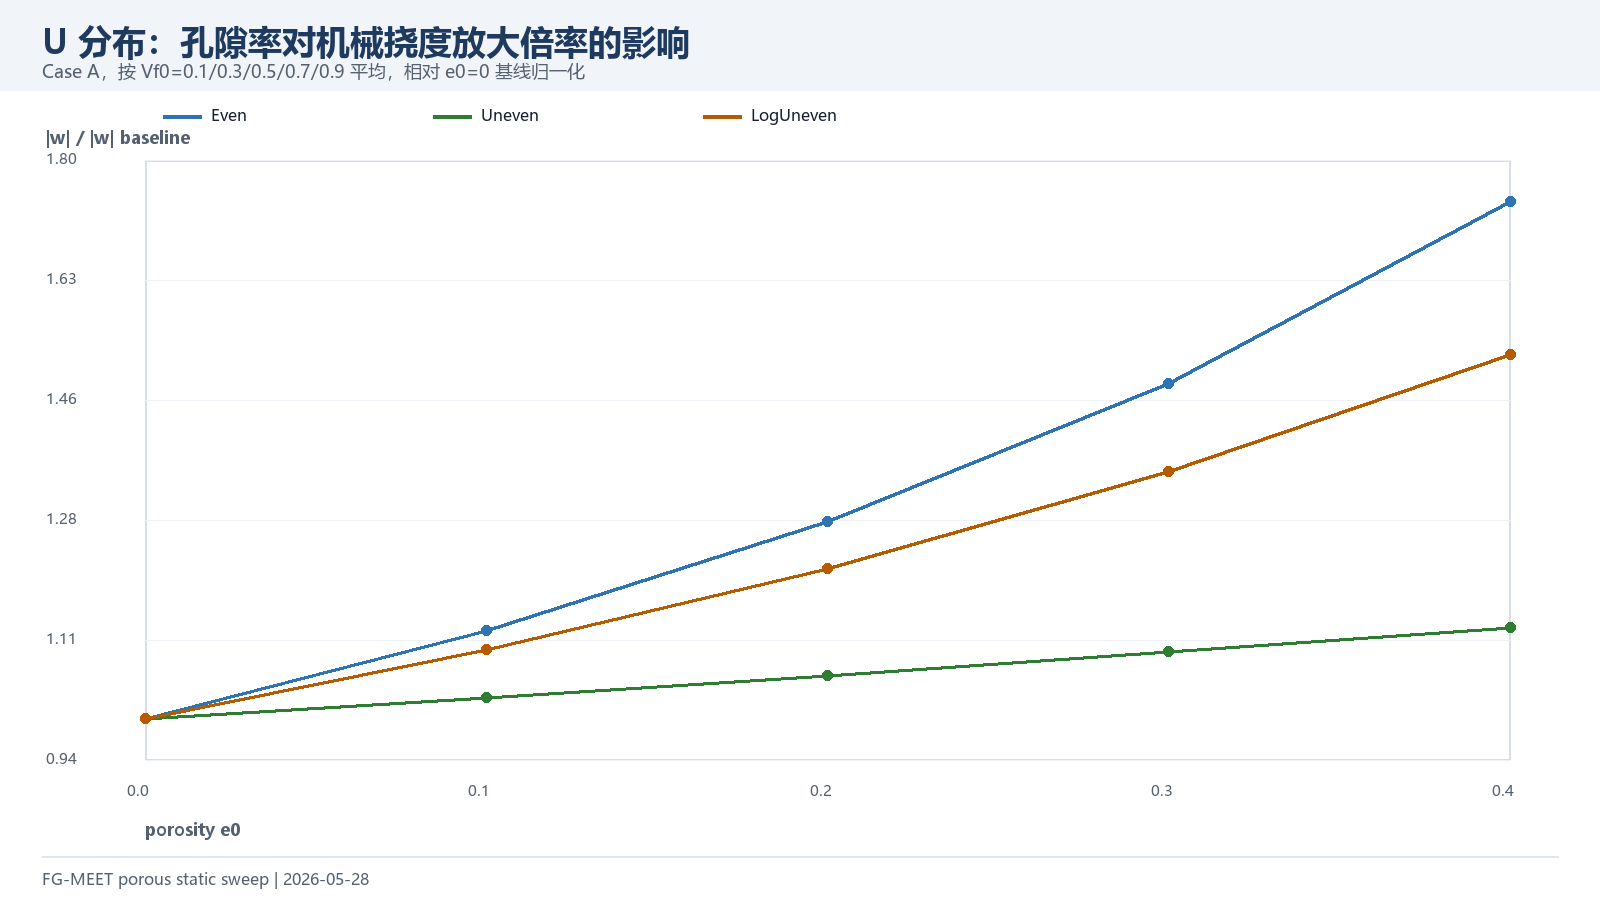
\includegraphics[width=\textwidth]{../reports/2026-05-28-porous-static/figures/02_U_elastic_deflection_ratio_vs_e0.png}
\caption{U 分布挠度倍率}
\end{subfigure}
\hfill
\begin{subfigure}{0.48\textwidth}
\centering
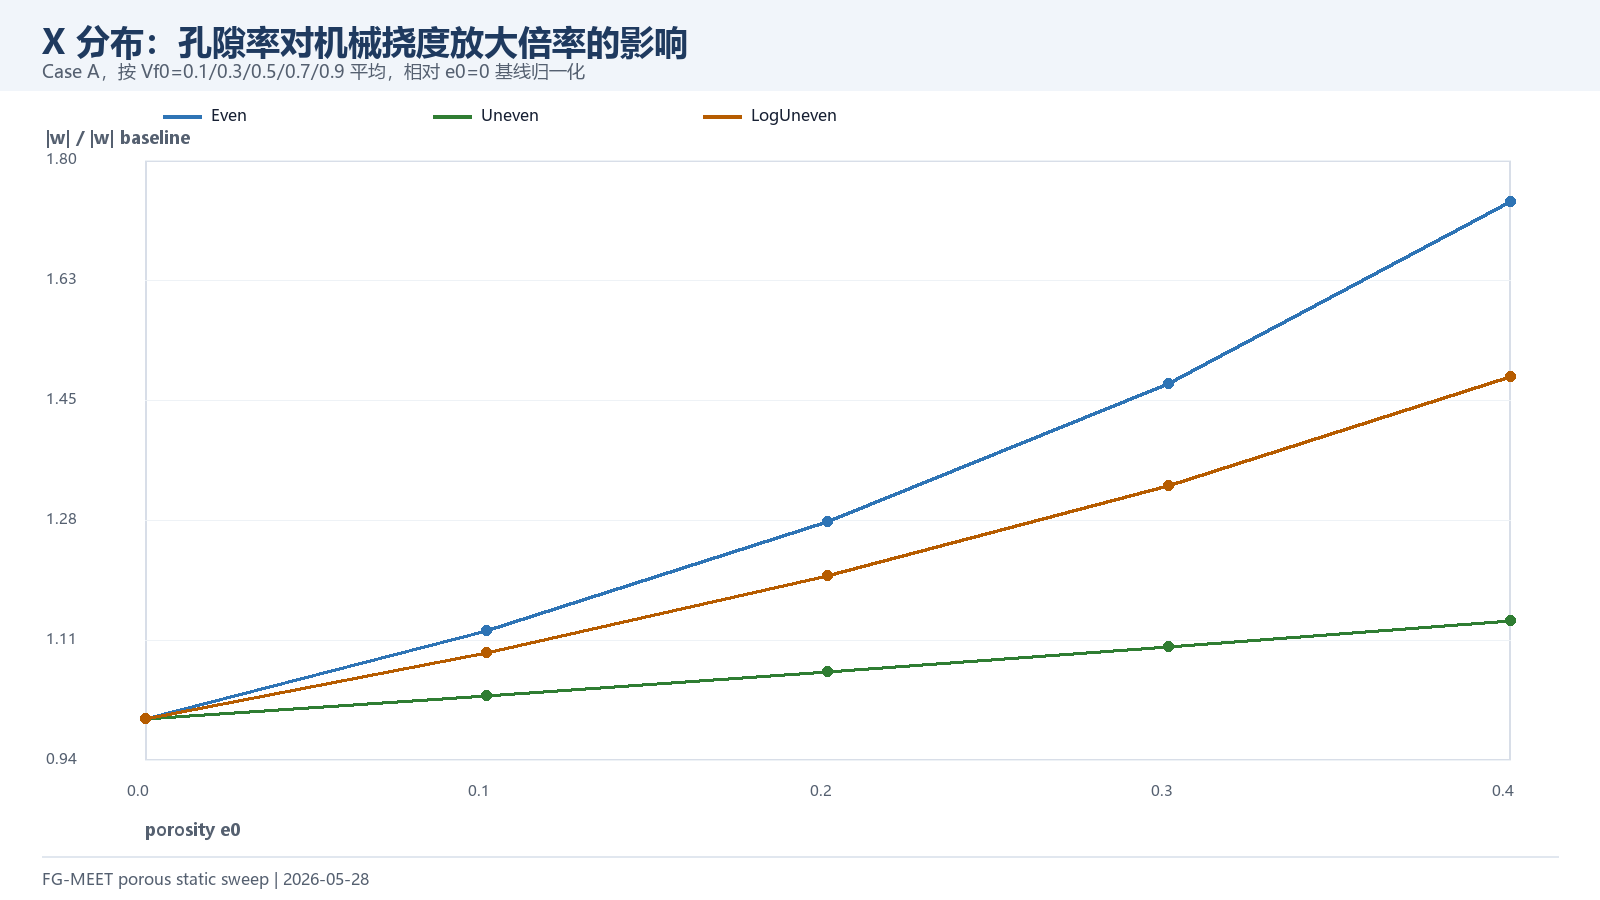
\includegraphics[width=\textwidth]{../reports/2026-05-28-porous-static/figures/02_X_elastic_deflection_ratio_vs_e0.png}
\caption{X 分布挠度倍率}
\end{subfigure}
\caption{孔隙率对 Case A 机械挠度放大倍率的影响}
\label{fig:porous-deflection-ratio}
\end{figure}

\begin{figure}[H]
\centering
\begin{subfigure}{0.48\textwidth}
\centering
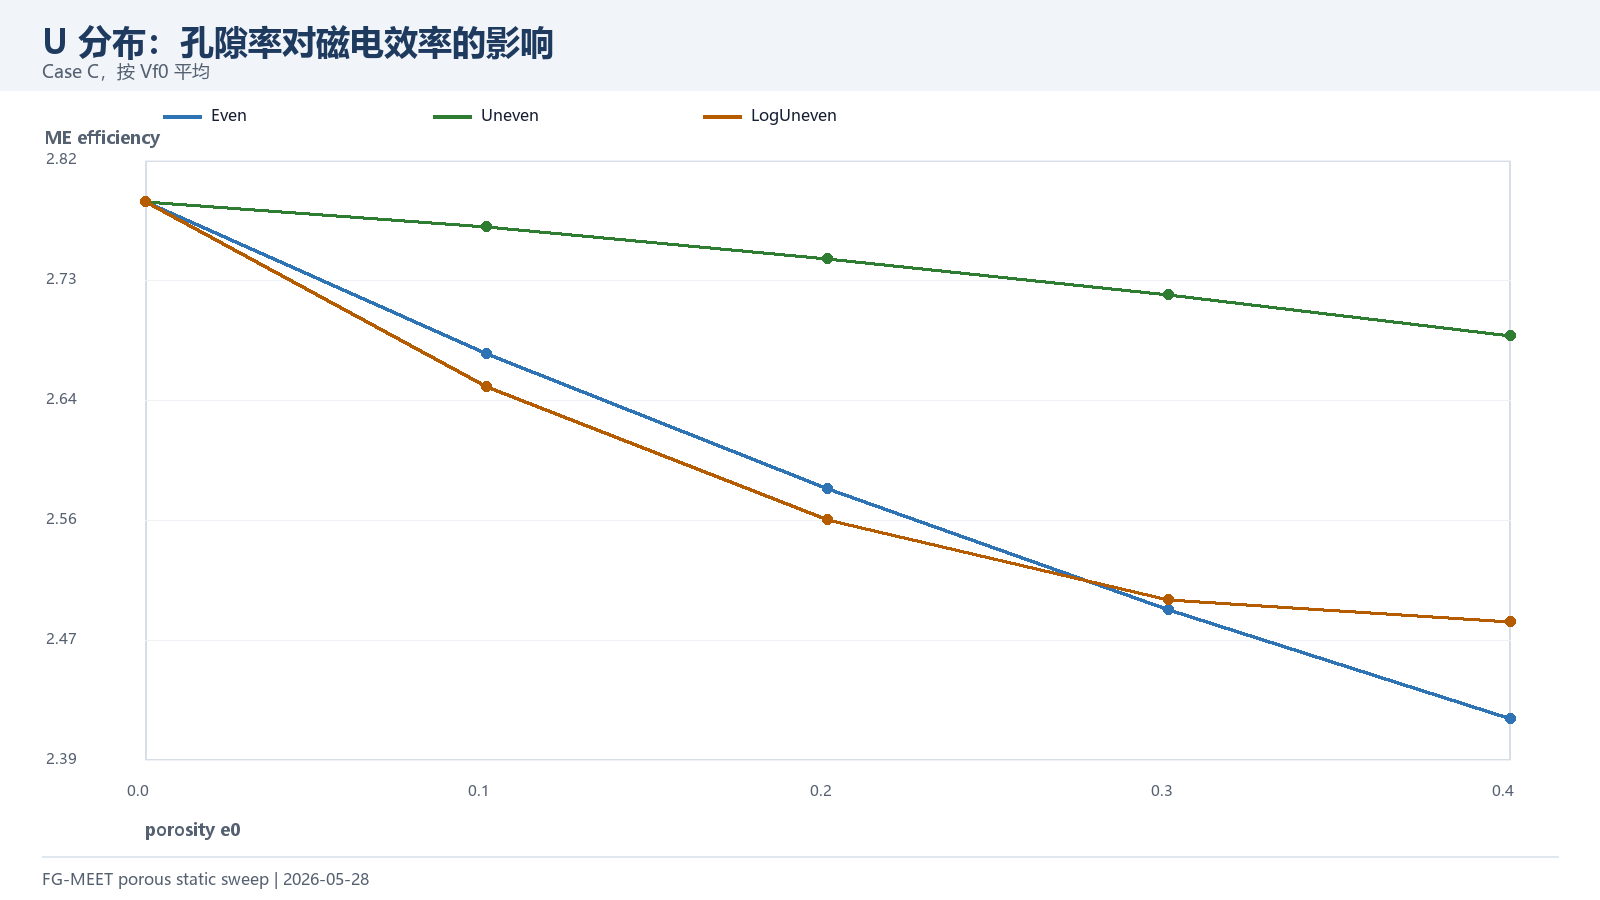
\includegraphics[width=\textwidth]{../reports/2026-05-28-porous-static/figures/04_U_me_efficiency_vs_e0.png}
\caption{U 分布磁电效率}
\end{subfigure}
\hfill
\begin{subfigure}{0.48\textwidth}
\centering
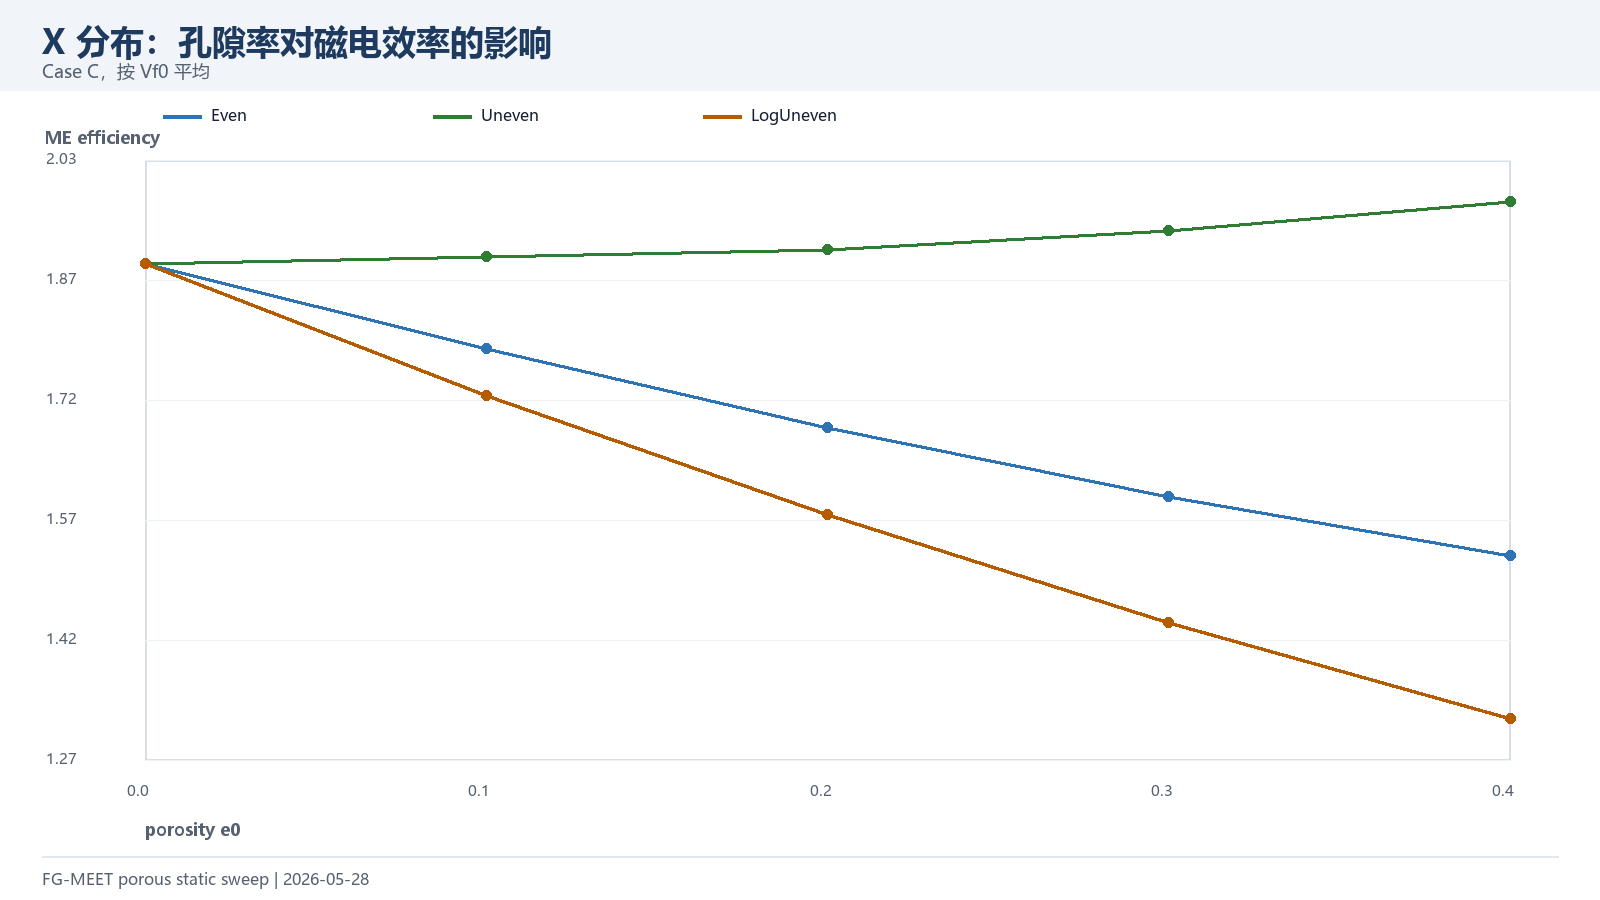
\includegraphics[width=\textwidth]{../reports/2026-05-28-porous-static/figures/04_X_me_efficiency_vs_e0.png}
\caption{X 分布磁电效率}
\end{subfigure}
\caption{孔隙率对 Case C 磁电效率的影响}
\label{fig:porous-me-efficiency}
\end{figure}

\subsection{边界条件影响（CFCF）}

为评估边界敏感性，补充了 CFCF（两对边固支）下的 $30\times30$ 扫描（U/X $\times$ 5 个 $V_{f0}$ $\times$ 3 载荷，共 30 行）。CFCF 相对 CFFF 强烈抑制中心挠度：机械载荷下最强抑制为 X/$V_{f0}=0.1$，CFCF/CFFF 挠度比 0.055；CFCF 最大机械挠度为 U/$V_{f0}=0.9$，$|w_{\text{center}}|=0.176$\,mm。CFFF 下确立的孔隙定性趋势（挠度放大、致动衰减）在 CFCF 下保持不变，仅绝对量级被更刚的边界整体缩小。

% ============================================================
\section{动力代表算例结果}
\label{sec:dynamic}
% ============================================================

瞬态分析按式~\eqref{eq:newmark} 的 Newmark-$\beta$ 格式在阶跃机械载荷下进行。由于 $30\times30$ 全量 Newmark 成本过高（见问题 P4），动力研究采用两个互补 pilot：用于 FG 分布与孔隙对比的 $10\times10$ 全量积分，以及用于验证降阶精度的 $30\times30$ 模态降阶。所有算例采用 0.1\,ms 时间步、40\,ms 窗口（401 步）、0.8\% Rayleigh 阻尼。

\subsection{无孔隙 FG 分布扫描（$10\times10$）}

$V_{f0}=0.6$ 下五种 FG 分布的 Case A 全量 Newmark 结果见表~\ref{tab:dyn-fg}。各分布中心挠度阶跃响应峰值约为静态值的两倍，超调比紧密集中于 2.10--2.14。O 型（中心富集）峰值最大（$-5.52$\,mm）、一阶频率最低（46.6\,Hz）；P 型（幂律）峰值最小（$-3.22$\,mm）、频率最高（62.9\,Hz）。一阶频率与各分布的静态刚度排序一致；X 型温差跨度最小（4.48\,K），与其表面富集特性带来的更均匀热响应一致。

\begin{table}[H]
\centering
\caption{无孔隙 $10\times10$ Newmark 动力结果（$V_{f0}=0.6$，CFFF，机械阶跃载荷）}
\label{tab:dyn-fg}
\small
\begin{tabular}{crrrrrc}
\toprule
\textbf{FG} & \textbf{静态} (mm) & \textbf{峰值} (mm) & \textbf{峰值时间} (ms) & \textbf{超调} & $f_1$ \textbf{(Hz)} & $\theta_{\max}$ \textbf{(K)} \\
\midrule
U & $-2.128$ & $-4.499$ & 28.9 & 2.114 & 52.20 & 5.129 \\
V & $-1.622$ & $-3.403$ & 25.0 & 2.098 & 60.91 & 5.374 \\
X & $-1.811$ & $-3.805$ & 26.3 & 2.101 & 57.62 & 4.480 \\
O & $-2.572$ & $-5.516$ & 32.8 & 2.144 & 46.57 & 6.101 \\
P & $-1.535$ & $-3.216$ & 39.7 & 2.096 & 62.93 & 5.316 \\
\bottomrule
\end{tabular}
\end{table}

\subsection{模态降阶验证（$30\times30$）}

$30\times30$ 网格（约 13800 自由度）保留前 8 阶模态叠加，静态捕获比 1.0004，给出 U/$V_{f0}=0.6$ 动力峰值 $-4.428$\,mm（对 $10\times10$ 全量 $-4.500$\,mm）。模态阶数敏感性研究（4/6/8/12/16 阶，表~\ref{tab:modal-sensitivity}）表明 16 阶峰值（$-4.427$\,mm）与 8 阶相差不足 0.001\,mm，证实 8 阶已收敛；阻尼比敏感性研究（$0$--$1.5\%$）将峰值限定在 $-4.504$\,mm（无阻尼）至 $-4.386$\,mm（$1.5\%$）之间，默认 0.8\% 给出 $-4.427$\,mm。

\begin{table}[H]
\centering
\caption{$30\times30$ 模态阶数敏感性分析}
\label{tab:modal-sensitivity}
\begin{tabular}{crrrrr}
\toprule
\textbf{阶数} & \textbf{捕获比} & \textbf{峰值 (mm)} & \textbf{峰值时间 (ms)} & \textbf{超调} & $\theta_{\max}$ \textbf{(K)} \\
\midrule
4  & 1.000349 & $-4.4281$ & 9.50 & 1.930 & 5.026 \\
6  & 1.000053 & $-4.4271$ & 9.60 & 1.929 & 5.028 \\
8  & 1.000370 & $-4.4279$ & 9.50 & 1.930 & 5.040 \\
12 & 1.000361 & $-4.4278$ & 9.50 & 1.930 & 5.040 \\
16 & 0.999965 & $-4.4270$ & 9.60 & 1.929 & 5.036 \\
\bottomrule
\end{tabular}
\end{table}

\subsection{含孔隙动力 pilot}

含孔隙代表工况（U/$V_{f0}=0.5$/$e_0=0.2$/Even，CFFF，Case A）在 $10\times10$ 全量 Newmark 网格上运行：静态中心挠度 $-2.456$\,mm，动力峰值 $-5.222$\,mm（27.8\,ms），超调比 2.13，最大厚度温差 6.50\,K，一阶频率 54.62\,Hz。超调比（2.13）与无孔隙值（2.10--2.14）基本一致，表明引入孔隙不改变阶跃响应的定性特征——它仅重标静态与峰值幅值（二者均因刚度降低而增大），而动力放大因子保持不变。

\begin{figure}[H]
\centering
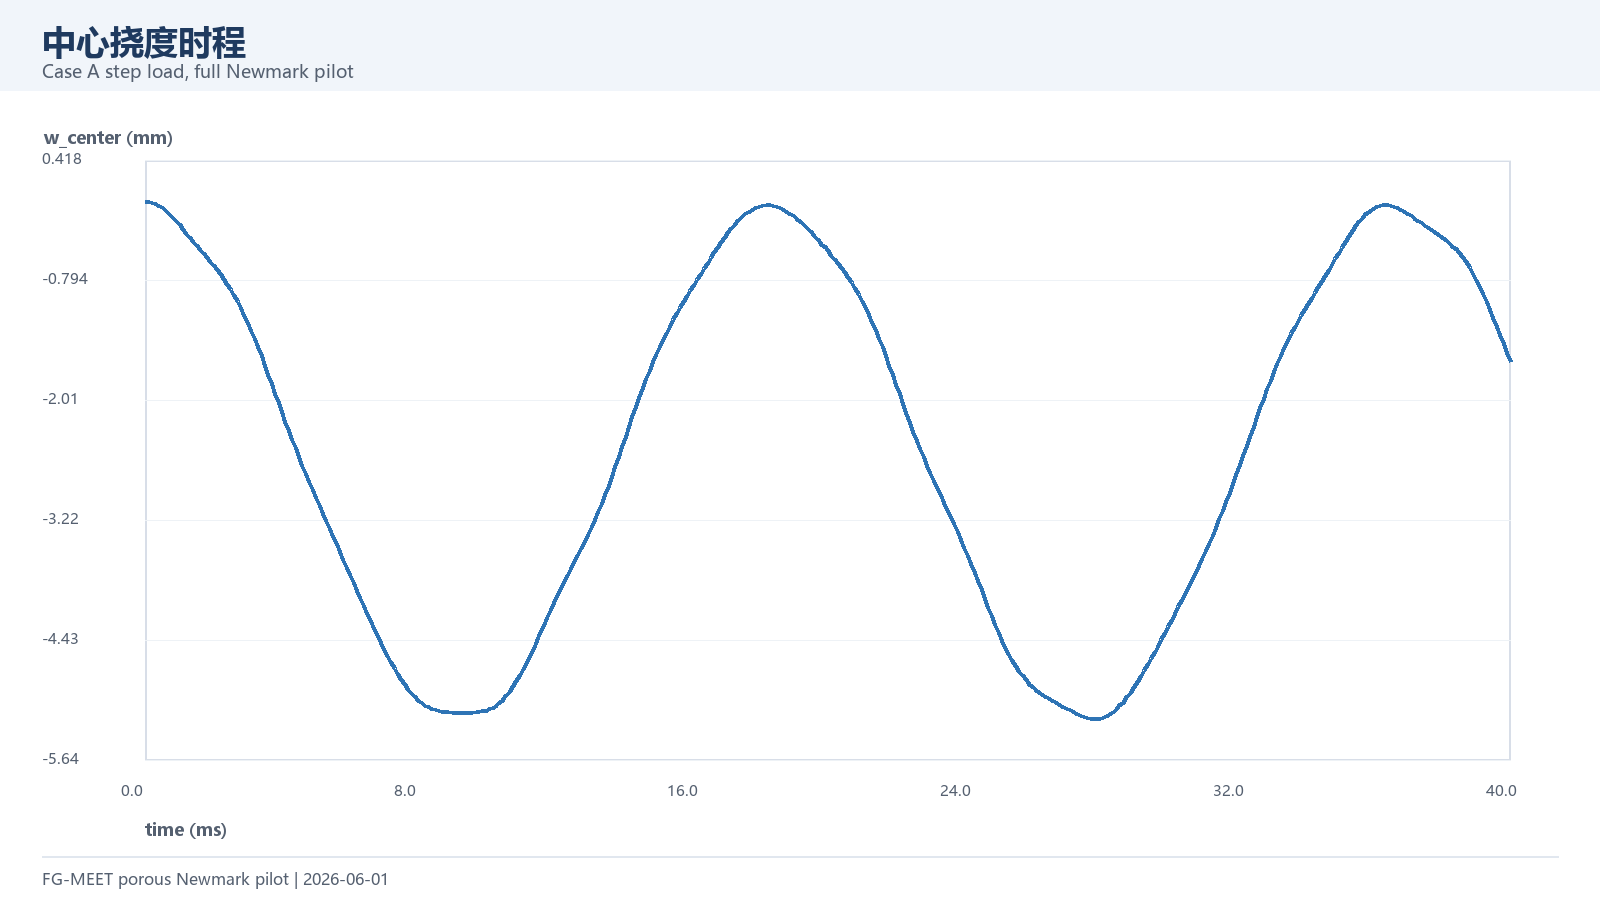
\includegraphics[width=0.7\textwidth]{../reports/2026-06-01-porous-dynamic/figures/02_porous_dynamic_center_timeseries.png}
\caption{含孔隙代表工况中心挠度时程（U/$V_{f0}=0.5$/$e_0=0.2$/Even）}
\label{fig:porous-dynamic-ts}
\end{figure}

由于本 pilot 与无孔隙扫描使用了不同体积分数（$V_{f0}=0.5$ 对 0.6），此处不直接比较二者频率；等 $V_{f0}$ 的含孔隙频率退化研究（$30\times30$ 模态网格）列为后续工作。

% ============================================================
\section{工作量总结}
% ============================================================

本研究完成的主要工作量与状态汇总于表~\ref{tab:summary}。

\begin{table}[H]
\centering
\caption{工作完成情况总结}
\label{tab:summary}
\begin{tabular}{p{5cm}cc}
\toprule
\textbf{任务} & \textbf{状态} & \textbf{关键指标} \\
\midrule
135 组无孔隙静力参数扫描 & \textcolor{passgreen}{完成} & 5FG$\times$9Vf$\times$3 载荷 \\
reduced $Q_d$ 还原修正（P1） & \textcolor{passgreen}{完成} & 135 行全部刷新 \\
2\,mm 耦合转化验证 & \textcolor{passgreen}{完成} & 6/6 pass \\
COMSOL 独立验证（无孔隙/非U/CFCF） & \textcolor{passgreen}{完成} & 最大误差 4.93\% / 4.19\% / 3.83\% \\
$10\times10$ 动力 pilot & \textcolor{passgreen}{完成} & 峰值 $-4.50$\,mm \\
$30\times30$ 模态降阶（P4） & \textcolor{passgreen}{完成} & 峰值 $-4.43$\,mm \\
模态阶数敏感性分析 & \textcolor{passgreen}{完成} & 8 阶已收敛 \\
阻尼比敏感性分析 & \textcolor{passgreen}{完成} & 0/0.5/0.8/1.5\% \\
含孔隙静力扫描 & \textcolor{passgreen}{完成} & 130 算例 / 390 行 \\
CFCF 边界补充扫描 & \textcolor{passgreen}{完成} & U/X 共 30 行 \\
含孔隙动力 pilot & \textcolor{passgreen}{完成} & $10\times10$ Newmark 401 步 \\
\midrule
含孔隙 COMSOL 代表验证 & \textcolor{warnblue}{需复核} & 中心 4.349--5.598\%，15点 5.434--6.594\% \\
含孔隙 $30\times30$ 模态 & \textcolor{warnblue}{待推进} & 等 $V_{f0}$ 频率退化 \\
\bottomrule
\end{tabular}
\end{table}

% ============================================================
\section{结论}
% ============================================================

本文采用基于一阶剪切变形理论的八节点 Serendipity 单元有限元模型，系统研究了含孔隙功能梯度磁--电--弹性板在热--磁--电--弹性全耦合载荷下的响应。将三种孔隙分布模型嵌入厚度梯度，在 130 配置（两种 FG 分布、五个体积分数、五个孔隙率、三种孔隙模式）设计空间下评估了力、电、磁三类载荷。主要结论如下：

\begin{enumerate}[leftmargin=2em]
\item \textbf{孔隙模式主导刚度退化。} $e_0=0.4$ 时 Even 孔隙使机械中心挠度放大约 74\%（$\sim1.74\times$），LogUneven 约 50\%，Uneven（中心富集）仅约 13\%。将孔隙集中于中面可保护弯曲关键的表层纤维，故 Uneven 即使在高孔隙率下也保留了大部分弯曲刚度。

\item \textbf{机械与致动响应对孔隙呈相反响应。} 机械载荷挠度随孔隙增大，而施加电压的压电致动挠度在 $e_0=0.4$ 时下降约 46\%（U/$V_{f0}=0.5$，Even）。结构上可容忍的孔隙会直接侵蚀主动致动能力，二者须作为耦合设计约束统一处理。

\item \textbf{相对刚度代价几乎与体积分数无关。} 在给定 FG/孔隙模式下，挠度放大倍率在 $V_{f0}=0.1$--$0.9$ 间变化不足 2\%；$V_{f0}$ 决定绝对量级，孔隙模式与水平决定相对代价。

\item \textbf{X 型梯度最小化变形诱导温升。} 表面富集 X 型在每个孔隙水平上厚度温差均小于 U 型（$e_0=0.4$ 时 3.85\,K 对 4.35\,K）。

\item \textbf{磁电效率随孔隙单调退化。} X 型 LogUneven 组合退化最强，$e_0=0.4$ 时损失 30.4\%；Uneven 模式最能保持效率。

\item \textbf{孔隙重标但不改变瞬态响应形态。} 阶跃超调比在无孔隙（2.10--2.14）与含孔隙（2.13）pilot 下均接近 2.1，引入孔隙改变静态与峰值幅值而不改变动力放大特征。
\end{enumerate}

\subsection*{局限与后续工作}

需说明若干局限：（i）宏观等效孔隙模型假设孔隙按比例缩放所有材料常数，不刻画孔形、连通性与尺寸分布；（ii）未能开展含孔隙 MEE 板的实验验证，MATLAB--COMSOL 交叉校核可缓解但不能替代实验确认。非均匀 FG 与 CFCF 的 COMSOL 行已满足 5\% 准则，但含孔隙代表行的中心点与 15 点最大偏差分别为 4.349--5.598\% 和 5.434--6.594\%，需要进一步复核模型构型；（iii）动力研究依赖 $10\times10$ pilot 与 $30\times30$ 模态降阶，完整的等 $V_{f0}$ 含孔隙频率退化分析留待后续；（iv）含孔隙空间仅纳入 U/X 两种梯度以控制成本，扩展至 V/O/P 分布及 CFCF 边界的全孔隙设计空间将使参数图谱更完整。

% ============================================================
\begin{thebibliography}{9}

\bibitem{nan2008multiferroic}
Nan, C.-W., Bichurin, M.~I., Dong, S., Viehland, D., Srinivasan, G., 2008.
Multiferroic magnetoelectric composites: Historical perspective, status, and future directions.
\textit{Journal of Applied Physics} 103 (3), 031101.

\bibitem{kondaiah2012studies}
Kondaiah, P., Shankar, K., Ganesan, N., 2012.
Studies on magneto-electro-elastic cantilever beam under thermal environment.
\textit{Smart Materials and Structures} 21 (3), 035000.

\bibitem{wattanasakulpong2014}
Wattanasakulpong, N., Ungbhakorn, V., 2014.
Linear and nonlinear vibration analysis of elastically restrained ends FGM beams with porosities.
\textit{Aerospace Science and Technology} 32 (1), 111--120.

\bibitem{zhao2024}
Zhao, Y., et al., 2024.
Thermoelastic analysis of porous functionally graded magneto-electro-elastic cylindrical shells.
\textit{Composite Structures} (in press).

\bibitem{zhang2026}
Zhang, et al., 2026.
Fully coupled thermo-magneto-electro-elastic finite element analysis of MEE plates: deformation-induced temperature field.
\textit{Manuscript / in-house formulation}.

\end{thebibliography}

\end{document}
